% !TEX TS-program = pdflatex
% !TEX encoding = UTF-8 Unicode

% This is a simple template for a LaTeX document using the "article" class.
% See "book", "report", "letter" for other types of document.

\documentclass[11pt]{article} % use larger type; default would be 10pt

\usepackage[utf8]{inputenc} % set input encoding (not needed with XeLaTeX)

%%% Examples of Article customizations
% These packages are optional, depending whether you want the features they provide.
% See the LaTeX Companion or other references for full information.

%%% PAGE DIMENSIONS
\usepackage{geometry} % to change the page dimensions
\geometry{a4paper} % or letterpaper (US) or a5paper or....
\geometry{margin=1in} % for example, change the margins to 2 inches all round
% \geometry{landscape} % set up the page for landscape
%   read geometry.pdf for detailed page layout information

\usepackage{graphicx} % support the \includegraphics command and options

% \usepackage[parfill]{parskip} % Activate to begin paragraphs with an empty line rather than an indent
\usepackage{amssymb}
\usepackage{amsmath}
%%% PACKAGES
\usepackage{booktabs} % for much better looking tables
\usepackage{array} % for better arrays (eg matrices) in maths
\usepackage{paralist} % very flexible & customisable lists (eg. enumerate/itemize, etc.)
\usepackage{verbatim} % adds environment for commenting out blocks of text & for better verbatim
\usepackage{subfig} % make it possible to include more than one captioned figure/table in a single float
% These packages are all incorporated in the memoir class to one degree or another...

%%% HEADERS & FOOTERS
\usepackage{fancyhdr} % This should be set AFTER setting up the page geometry
\pagestyle{fancy} % options: empty , plain , fancy
\renewcommand{\headrulewidth}{0pt} % customise the layout...
\lhead{}\chead{}\rhead{}
\lfoot{}\cfoot{\thepage}\rfoot{}

%%% SECTION TITLE APPEARANCE
\usepackage{sectsty}
\allsectionsfont{\sffamily\mdseries\upshape} % (See the fntguide.pdf for font help)
% (This matches ConTeXt defaults)

%%% ToC (table of contents) APPEARANCE
\usepackage[nottoc,notlof,notlot]{tocbibind} % Put the bibliography in the ToC
\usepackage[titles,subfigure]{tocloft} % Alter the style of the Table of Contents
\usepackage{bbm}
\usepackage{endnotes}

\renewcommand{\cftsecfont}{\rmfamily\mdseries\upshape}
\renewcommand{\cftsecpagefont}{\rmfamily\mdseries\upshape} % No bold!
\DeclareMathOperator*{\argmax}{arg\,max}
\DeclareMathOperator*{\argmin}{arg\,min}

\usepackage{graphicx}
\graphicspath{ {./pings/} }

\newcount\colveccount
\newcommand*\colvec[1]{
        \global\colveccount#1
        \begin{pmatrix}
        \colvecnext
}
\def\colvecnext#1{
        #1
        \global\advance\colveccount-1
        \ifnum\colveccount>0
                \\
                \expandafter\colvecnext
        \else
                \end{pmatrix}
        \fi
}

\newcommand{\norm}[1]{\left\lVert#1\right\rVert}

\title{Econometrics HW2}
\author{Michael B. Nattinger\footnote{I worked on this assignment with my study group: Alex von Hafften, Andrew Smith, and Ryan Mather. I have also discussed problem(s) with Emily Case, Sarah Bass, Katherine Kwok, and Danny Edgel.}}

\begin{document}
\maketitle

\section{Question 18.2}
\subsection{Part A}
This is essentially just a regression of $Y$ on $D$ with state fixed effects, so the estimator is the following:
\begin{align*}
\hat{\theta} &= \frac{\sum_{t=0}^{T}\sum_{i=0}^{N}(D_{it} - \bar{D}_{i})(Y_{it} - \bar{Y}_{i})}{\sum_{t=i}^{T}\sum_{i=1}^{N}(D_{it} - \bar{D}_{i})^2},
\end{align*}
where $\bar{D}_i = (1/T)\sum_{t=1}^T D_{it},\bar{Y}_i = (1/T)\sum_{t=1}^T Y_{it}$.
\subsection{Part B}
For the untreated sample, $D_{it} = 0 \forall t,$ so $D_{it} - \bar{D}_i = 0 \forall t,$ so $\hat{\theta} =  \frac{\sum_{t=0}^{T}\sum_{i=0}^{N}(D_{it} - \bar{D}_{i})(Y_{it} - \bar{Y}_{i})}{\sum_{t=0}^{T}\sum_{i=0}^{N}(D_{it} - \bar{D}_{i})^2} =  \frac{\sum_{t=0}^{T}(D_{1t} - \bar{D}_{1})(Y_{1t} - \bar{Y}_{1})}{\sum_{t=0}^{T}(D_{1t} - \bar{D}_{1})^2}$ which is a function only of the treated sample.
\subsection{Part C}
No, it is only a difference estimator of the treated group. It is not accounting for the control group, as shown from the independence result from Part B.
\subsection{Part D}
If the time trend is not important then the control group would have no change over time, so the difference estimator would be the same as the difference-in-difference estimator.
\section{Question 18.4}
For both, if all interaction dummies were included then there would be perfect collinearity and the $X'X$ matrix would not be invertible. Intuitively one of the groups serve as a baseline from which the other groups are compared.
\section{Question 18.5}
\subsection{Part A}
The difference in Wisconsin is $16.72 - 15.23 = 1.49$. The difference in Minnesota is $18.10-16.42 = 1.68$. The difference in difference estimate is therefore $1.49 - 1.68 = -0.19$.
\subsection{Part B}
$\hat{\beta} = -0.1$.
\subsection{Part C}
$\hat{\gamma} = 15.23 - 16.42 = -1.19.$

\section{Question 17.1}
\subsection{Part A}
We will integrate and make a variable substitution $y = \frac{X_i - x}{h}\Rightarrow h dy = dx$
\begin{align*}
E[X^*] &= \int x \frac{1}{nh} \sum_{i=1}^n K((X_i - x)/h) dx\\
&= \frac{1}{nh}\sum_{i=1}^n \int x K((X_i - x)/h) dx \\
&= \frac{1}{n}\sum_{i=1}^n \int (X_i - hy) K(y) dy  \\
&= \frac{1}{n}\sum_{i=1}^n X_i \int K(y) dy - \frac{h}{n}\sum_{i=1}^n \int y K(y) dy \\
&= \frac{1}{n}\sum_{i=1}^n X_i \\
&= \bar{X}_n,
\end{align*}
where we have used the fact that the kernels integrate to 1 and have mean 0.
\subsection{Part B}
We will again ust the same substitution.
\begin{align*}
Var(X^*) &= E[X^{*2}] - E[X^*]^2\\
&= \int x^2 \frac{1}{nh} \sum_{i=1}^n K((X_i - x)/h) dx -\bar{X}_n^2 \\
&= \frac{1}{n}\sum_{i=1}^N \int (X_i-hy)^2K(y)dy -\bar{X}_n^2\\
&= \frac{1}{n}\sum_{i=1}^N X_i^2 \int K(y)dy - \frac{2h}{n}\sum_{i=1}^N X_i \int yK(y)dy + \frac{h^2}{n}\sum_{i=1}^N \int y^2K(y)dy -\bar{X}_n^2\\
&= \frac{1}{n}\sum_{i=1}^N X_i^2  + h^2 - \bar{X}_n^2\\
&= \hat{\sigma}^2 + h^2.
\end{align*}
\section{Question 17.3}
The optimal bandwidth is $h_0 = \left(\frac{R_K}{R(f'')}\right)^{1/5}n^{-1/5}$. Note that, for a uniform distribution, $f'' = 0 \Rightarrow R(f'') = 0.$ The optimal bandwidth is the largest feasible bandwidth.
\section{Question 17.4}
The effective bandwidth would be much larger as the scale was reduced by a factor of $10^6$ yet the bandwidth was unchanged. The plot would be much wider, smoother, and lower than it should be. 

If the bandwidth was scaled appropriately by $1000000^{-1}$ when the scale changed, the density plots would have the same shape.
\section{Question 19.3}
When $m(x)$ is increasing and convex, the bias is positive. When $m(x)$ is increasing and concave, the bias is negative. When $m(x)$ is decreasing and concave, the bias is again negative. When $m(x)$ is decreasing and convex, the bias is positive. The intuition here is that you are locally averaging around a point of interest. This is similar to taking the midpoint of a function over a region of concavity or convexity.

Moreover, asymptotic theory tells us that the bias is $\frac{1}{2}m''(x)h^2$ and $m''(x)>0$ for a convex function and $m''(x)<0$ for a concave function.
\section{Question 19.4}
Bias is $B(x) = (1/2) m''(x)+ m'(x)f'(x)/f(x) = \beta f'(x)/f(x)$. If $\beta>0,$ then $b(x)<0 \iff f'(x)<0,$ $b(x)>0 \iff f'(x)>0.$ In contrast, if $\beta<0$ then $b(x)<0 \iff f'(x)>0,$ $b(x)>0 \iff f'(x)<0.$

$f(x)$ is the marginal density of $X$. If $f'(x)>0$ then the density of $X$ is increasing at $x$, so if $\beta$ is positive (negative),  the bias at $x$ is positive because it is influenced more by the mass of $X$ to the right of $x$, so the positive (negative) influence of this mass on the conditional expectation due to the positive (negative) value of $\beta$ leads to a positive (negative) bias.
\section{Question 19.9}
\subsection{Part A}
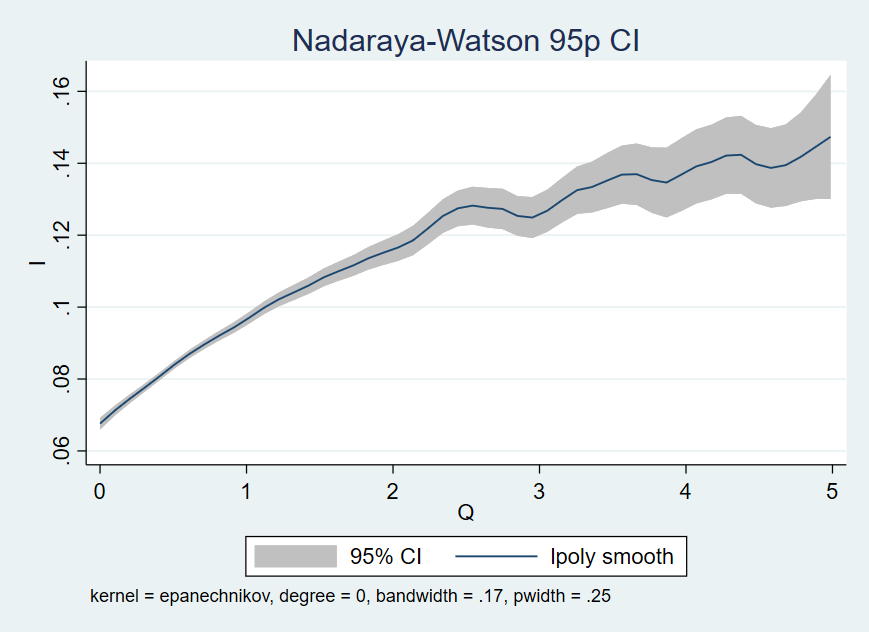
\includegraphics[scale=0.5]{9p1}
\subsection{Part B}
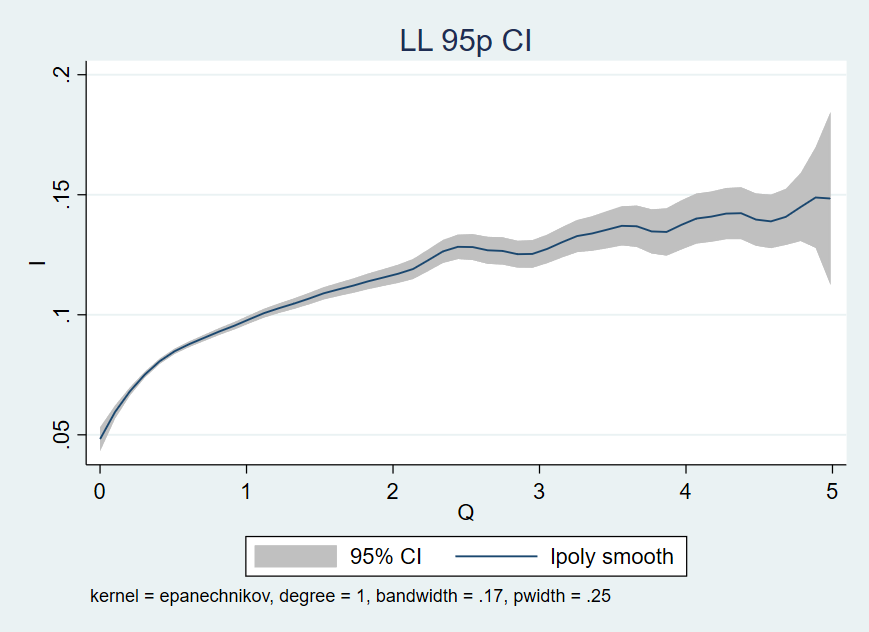
\includegraphics[scale=0.5]{9p2}
\subsection{Part C}
Yes, from the graphs in the preceding parts of this question it appears that there is nonlinearity in the relationship.

Stata code:

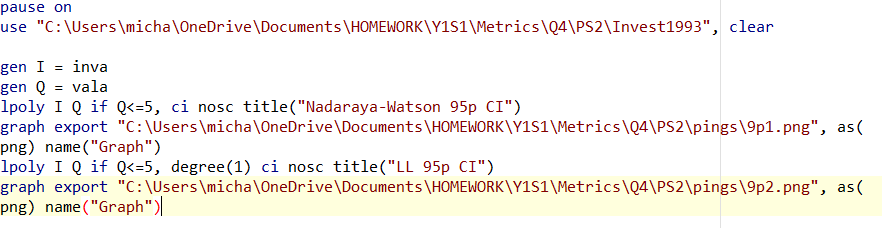
\includegraphics[scale=0.7]{code9}
\section{Question 19.11}
\subsection{Part A}
Done in stata, see code below the final part of this question.
\subsection{Part B}
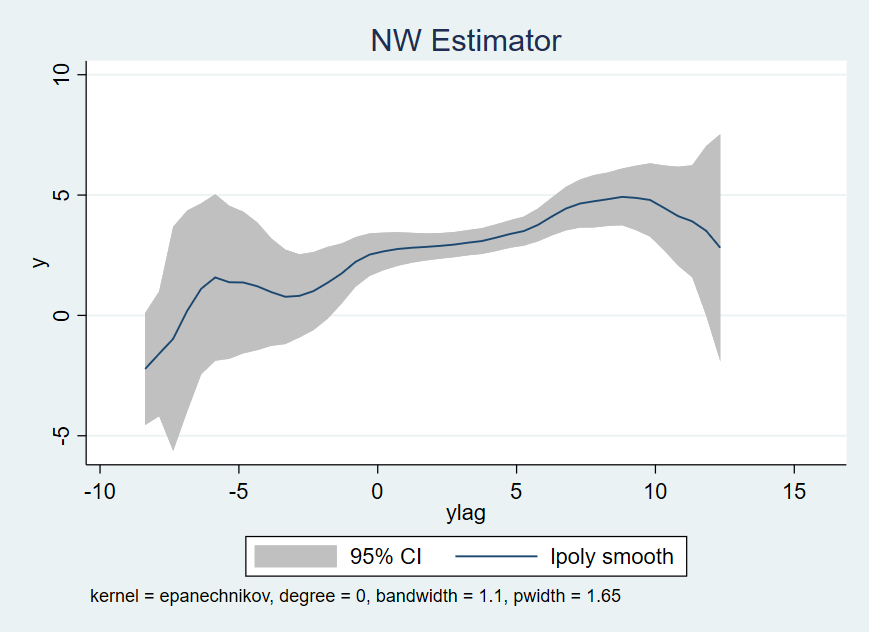
\includegraphics[scale=0.5]{11p1}
\subsection{Part C}
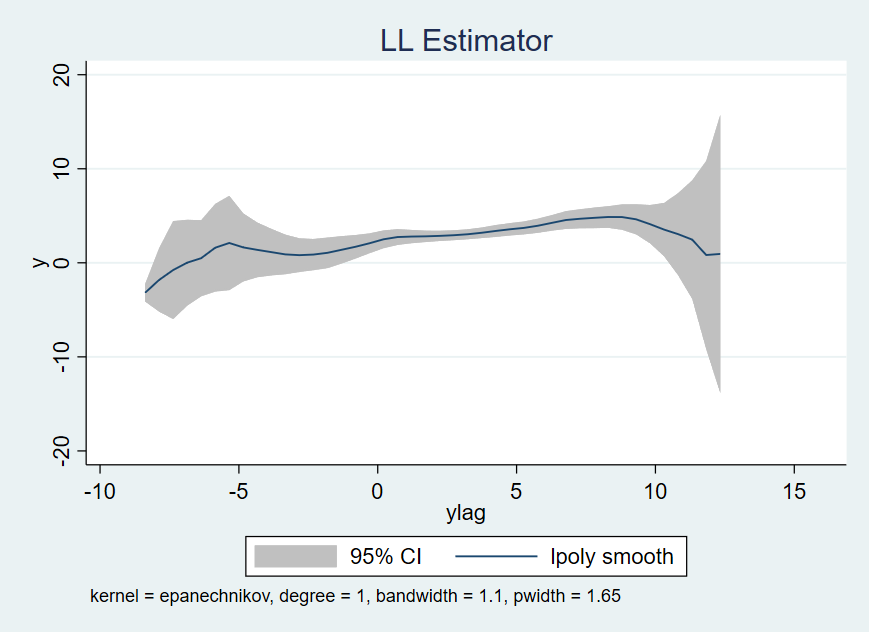
\includegraphics[scale=0.5]{11p2}
\subsection{Part D}
Yes, from the graphs in the preceding parts of this question it appears that there is nonlinearity in the relationship.

Stata code:

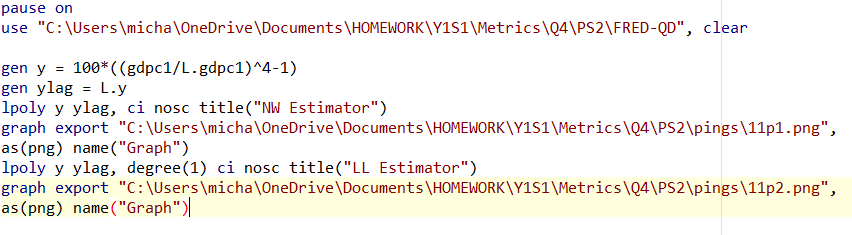
\includegraphics[scale=0.7]{code11}

\end{document}
